\documentclass [a4paper, 11pt]{article}

\usepackage{amsmath,amssymb}
\usepackage{epsfig}
\usepackage{graphicx}
\usepackage{times}
\usepackage{float}
\usepackage[usenames,dvipsnames]{color}
\usepackage{hyperref}
\usepackage{scrlayer-scrpage}
\usepackage{subfigure}
\usepackage{cleveref}
\usepackage{bm}
\pagestyle{scrheadings}
\clearpairofpagestyles

\textwidth 16 cm
\textheight 23 cm
\setlength{\oddsidemargin}{0.1 cm}
\setlength{\topmargin}{1 cm}
\setlength{\headheight}{0cm}
\setlength{\headsep}{0cm}
\setlength{\footskip}{0.75cm}
\setlength{\parindent}{0cm}
\setlength{\oddsidemargin}{0.1 cm}
\setlength{\itemsep}{10pt}
\bibliographystyle{gcs}
\cfoot{\pagemark}
\ofoot{\tiny V1.9-2022JUL06}

\newcommand{\Pvec}{\mathbf{P}}

\begin{document}

\LARGE
\begin{center}
	\bf Project Report\\
\end{center}

\large
\bigskip
\bigskip
\bigskip

\textbf{Type of report}\\
\phantom{MM}\textit{“Status Report”}

\bigskip
\textbf{Period}\\
\phantom{MM}\textit{10.2023-9.2024}

\bigskip
\textbf{Project title}\\
\phantom{MM}\textit{Inclusive semileptonic decay rates from lattice QCD}

\bigskip
\textbf{HPC system(s) and corresponding centres(s)}\\
\phantom{MM} \textit{JUWELS Booster, JSC}

\bigskip
\textbf{Project ID}\\
\phantom{MM} \textit{ISDLQCD}

\textbf{Principal investigator}\\
\phantom{MM} \textit{C. Urbach, Helmholtz-Institut für Strahlen- und Kernphysik (Theorie) and
	Bethe Center for Theoretical Physics, University of Bonn, 53115 Bonn, Germany}

\bigskip
\textbf{Project contributor(s)}\\

\phantom{MM} \textit{
	A.~Evangelista$^a$,
	R.~Frezzotti$^a$,
	G.~Gagliardi$^b$,
	M.~Garofalo$^c$,
	C.~Groß$^c$,
	B.~Kostrzewa$^d$,
	V.~Lubicz$^e$,
	M.~Panero$^f$,
	F.~Sanfilippo$^b$,
	S.~Simula$^b$,
	A~Smecca$^g$,
	N.~Tantalo$^a$
}\\


\textit{$^a$ Dipartimento di Fisica and INFN, Universit\`a di Roma ``Tor Vergata", Via della Ricerca Scientifica 1, I-00133 Roma, Italy}\\
\textit{$^b$ Instituto Nazionale di Fisica Nucleare, Sezione di Roma Tre, Via della Vasca Navale 84, I-00146 Rome, Italy }\\
\textit{$^c$ Helmholtz-Institut f{\"u}r Strahlen- und Kernphysik (Theorie) and Bethe Center for Theoretical Physics, Universit{\"a}t Bonn}\\
\textit{$^d$ High Performance Computing and Analytics Lab, University of Bonn, 53115 Bonn, Germany} \\
\textit{$^e$ Dipartimento di Matematica e Fisica, Universit\`a Roma Tre and INFN, Sezione di Roma Tre, Via della Vasca Navale 84, I-00146 Rome, Italy} \\
\textit{$^f$ Dipartimento di Fisica, Università di Torino \& INFN, Sezione di Torino, Via Pietro Giuria 1, I-10125 Turin, Italy}\\
\textit{$^g$ Department of Physics, Faculty of Science and Engineering, Swansea University (Singleton Park Campus) Singleton Park, SA2 8PP Swansea, Wales, United Kingdom}

\newpage

\vfill
\tableofcontents
\vfill

\newpage

\section{Abstract}\label{sec:abstract}
\rule{\textwidth}{0.4pt}
%\textit{Give a short introduction to the project and stress the highlights.}\\


Flavour physics is an important and active research topic, it has high potential
for the discovery of a statistically significant discrepancy between the SM and
experiment.
Even if the mass scales of new
particles beyond the SM turned out to be very high, quantum effects of
the associated fields could leave detectable imprints on the physics
of heavy quarks.
This indicates the need for precise theoretical computations from
first principles of observables related to semi-leptonic decays of
heavy mesons and elements of the CKM matrix. 

With the computer time granted to us in the current granting period we
were able to perform a fully non-perturbative computation of the inclusive semileptonic
decay rate of the $D_s$ meson.
A first principles computation of this decay rate is of high
phenomenological relevance, since a comparison with experimental data
allows for stringent Standard Model tests in the sector of Flavour physics.
Additionally, our work sets the stage to a future
project involving the $B$ meson(s), which will allows us to
investigate current flavour anomalies.



\section{Scientific work accomplished and results obtained}\label{sec:results}
\rule{\textwidth}{0.4pt}

In the current accounting period we were so far able to run the
proposed jobs according to our schedule. Since the granted computing
time was less than what we proposed, we had changed our plan
accordingly.
However, by reducing our target the statistics from 400 gauge
configurations per ensemble to 300, and by reducing the
number of stochastic sources by a factor two,
% and using other time 
% available to us in other machines (LEONARDO booster at CINECA)
we could
generate enough data to perform our calculation, while slightly
sacrificing the statistical precision. 
% However, due to extra time available to us due to JUWELS
% being idle otherwise, we could nevertheless generate according to plan.

The gauge ensembles we use to generate data are compiled in Table~\ref{tab:ensembles}.
With respect to our proposal, we replace the ensemble cAp211.077.64
with the cB211.072.48, the latter being computationally
cheaper. However, with this change we have three ensembles with all
parameteres but the volume equal, which provides us with very valuable
insights into finite volume effects.

With this improved control over finite volumen effects, we have also
replaced ensemble cC211.06.112 with cE211.044.112. Both 
ensembles come with similar computational costs, but the cE211.044.112
is at a finer lattice spacing allowing us to perform a better
controlled continuum limit, while finite volume effects are controlled
by the three cB ensembles.

There are some runs that we still need to perform, however, the
accounting period is also not yet over.


\begin{table}[h]
	\centering % center the table
	\begin{tabular}{lccccr} % alignment of each column data
		\hline
		name          & $L$ [fm]      & $a$
		[fm]          & $M_\pi$ [MeV] & $M_\pi L$                         \\
		\hline
		% cAp211.077.64 & 5.76 & $\sim$0.09 & $\approx$ 135 & 3.95  \\
		\hline
		cB211.072.48  & 3.84          & $\sim$0.08 & $\approx$ 135 & 2.63 \\
		cB211.072.64  & 5.12          & $\sim$0.08 & $\approx$ 135 & 3.51 \\
		cB211.072.96  & 7.68          & $\sim$0.08 & $\approx$ 135 & 5.27 \\
		\hline
		cC211.06.80   & 5.44          & $\sim$0.07 & $\approx$ 135 & 3.72 \\
		% cC211.06.112  & 7.62          & $\sim$0.07 & $\approx$ 135 & 5.21 \\
		\hline
		cD211.054.96  & 5.76          & $\sim$0.06 & $\approx$ 135 & 3.94 \\
		\hline
		cE211.044.112 & 5.48          & $\sim$0.05 & $\approx$ 135 & 3.75 \\
		\hline
	\end{tabular}
	\caption{ETMC's $N_f=2+1+1$ gauge ensembles relevant for this
		proposal. The time extent is always set to $T=2L$.}
	\label{tab:ensembles}
\end{table}

\subsection{Sub-project 1: Total inclusive decay rate $D_s \to X\ell\nu$}

The total inclusive decay rate for the
process $D_s \to X\ell\nu$ can be written as
\begin{equation}
	\Gamma = G^2_F\left\{ |V_{cd} |^2 \Gamma_{cd} + |V_{cs} |^2 \Gamma_{cs} + |V_{us} |^2 \Gamma_{su}
	\right\}\,,
\end{equation}
where the different contributions on the right hand side correspond at the quark level to the weak
transitions $c \to d$, $c \to s$, and $s \to u$, respectively.
The contribution $su$ is suppressed by the integration over the phase
space thus expected to be negligible. So far, we have computed only
the contribution coming from the channels $cd$ and $cs$ and the
computaiton of the $su$ channel is still ongoing.
Each term can be computed
\begin{equation}
	\frac{48 \pi^4}{m_{B_{(s)}}^5}\frac{d\Gamma_{fg}}{d \bm{ q^2} }
	=\lim_{\sigma\to 0}\sum_{l=0}^2 |\bm{q}|^{3-l}\int_0^{\infty}d q_0 (q^{max}_0-q_0)^l\Theta_\sigma(q_0^{max},q_0) Z^l\,.
	\label{eq:gamma}
\end{equation}
The above integral can be computed with the HLT method \cite{Hansen:2019idp} reconstructing the
convolution of the spectral
density $Z$  with the kernel $\Theta_\sigma$.
In the HLT method, the kernel $\Theta_\sigma$ gets replaced by an
approximate kernel $\sum_{\tau=1}^Ng_\tau e^{-\omega_0\tau}$, where
$N$ is the number of time slices used in the spectral recontruction,
and $g$ are parameters to be determined minimizing the function 
\begin{equation}
  W[\lambda, g]=(1-\lambda)\frac{A[g]}{A[0]}+\lambda B[g]\,.
  \label{eq:W_HLT}
\end{equation}
The systematic error in approximating the kernel is given by
$A[g]=\int_{E_0}^\infty d \omega_0( \sum_{\tau=1}^N g_\tau e^{-\omega_0\tau}- \Theta_\sigma )^2$
and the statistical error by $B[g]=\bm{g}^T
\mbox{COV}[C(t)]\bm{g}$ with correlator $C(t)$. $\lambda$ represents a
trade-off of parameter to balance systematic versus statistical
error. The effect of $\lambda$ on the decay rate is shown in
Figure~\ref{fig:stability}, where we see that there is a window in
$\lambda$ where the result is stable. 

\begin{figure}
  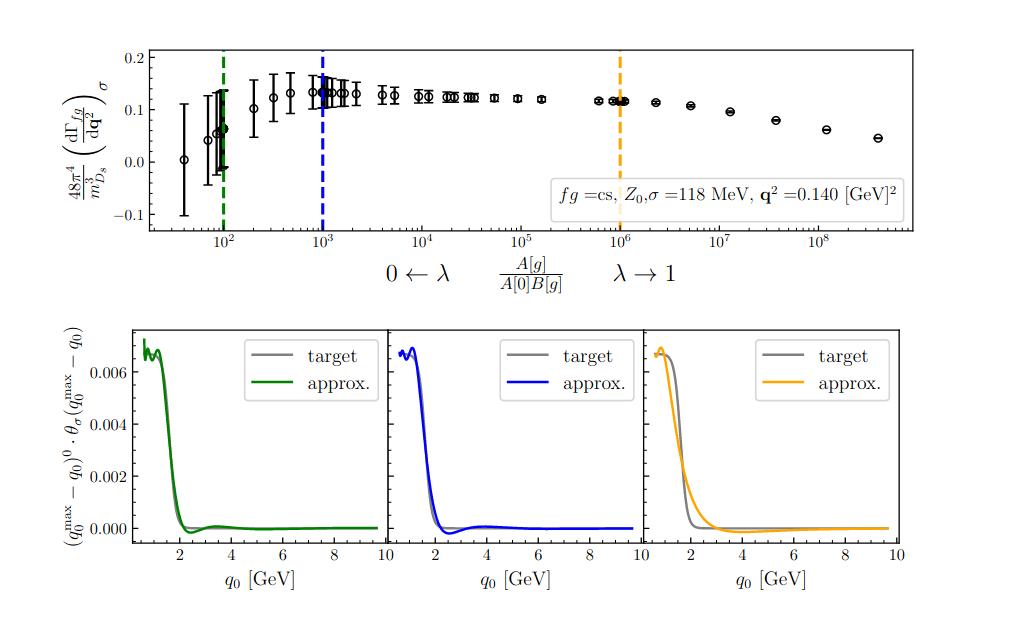
\includegraphics[scale=0.5]{figures/Screenshot from 2024-07-27 18-12-04.png}
  \caption{Values of the decay width obtained from different values of $\lambda$, the trade-off
    parameter of Eq.~\ref{eq:W_HLT} in the top panel. In the panels below we show the kernel $\Theta_\sigma$ against the kernel reconstructed from the HLT method at the values of  $\lambda$ corresponding to
    marked by vertical dashed lines in the panel above.
  }
  \label{fig:stability}
\end{figure}

% with the data produced we also observed that 
% our calculation the  extrapolation $\sigma \to 0$ can been done 
Another central point in our project is the $\sigma \to 0$
extrapolation. As visible in Figure~\ref{fig:sigma_extrapolation}, the
$\sigma \to 0$ extrapolation is smooth and can be described by 
a polynomial function in $\sigma$.

\begin{figure}
  \centering
  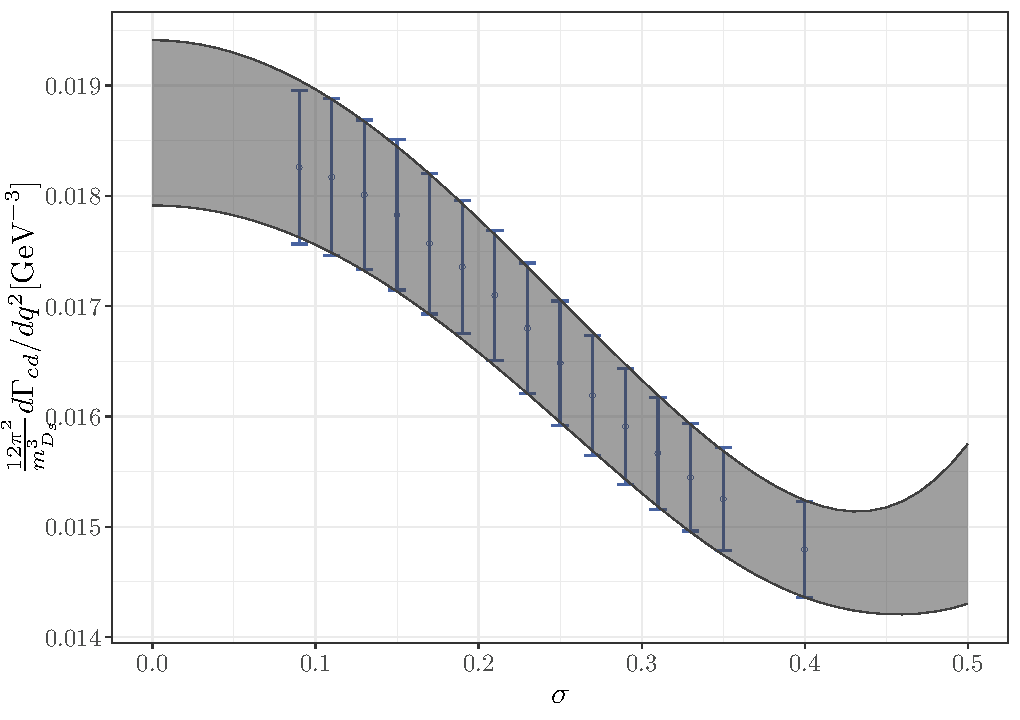
\includegraphics[scale=0.5]{figures/sigma_extrapolation.pdf}
  \caption{ $\sigma \to 0 $ extrapolation for the decay width in the channel $cu$.
  }
  \label{fig:sigma_extrapolation}
\end{figure}

For the total inclusive decay rate $D_s \to X\ell\nu$, the usage of three volumes
at the same lattice spacing (cB211.072.48, cB211.072.64 and cB211.072.96)
gives us control over the finite volume effects. As we can see in Fig.~\ref{fig:dGamma_FSE_B},
there is no sign of finite volume effects with the present statistical
uncertainty, which is the main reason for the aforementioned
replacement of ensemble cC211.06.112 with the finer lattice spacing
ensemble cE211.044.112.
An example for the continuum limit of the differential decay rate at
$q^2=0.7\,\mathrm{GeV}^2$ is shown in Figure~\ref{fig:dGamma_continuum}. We find that the
$\mathbf{O}(a^2)$ lattice artefacts are compatible with a constant
fit. The ensemble cC211.06.112, responsible for the second data point
from the right, though likely requires more statistic as we observe from Figure~\ref{fig:dGamma_continuum}.

\begin{figure}
	\begin{center}
		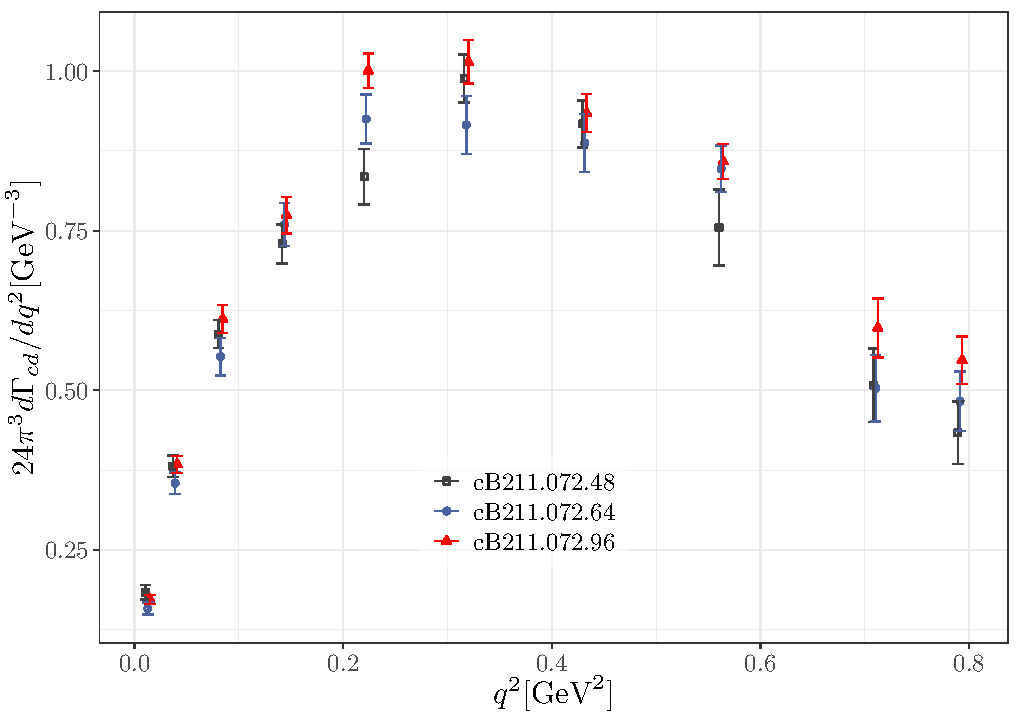
\includegraphics[scale=0.7]{figures/dGamma_FSE_B.pdf}
		\caption{Values of $d\Gamma_{cd}/dq^2 $ for the channel $cd$ obtained at three different volume
			ensembles with the same lattice spacing, the ensembles are cB211.072.48, cB211.072.64 and cB211.072.96.}
		\label{fig:dGamma_FSE_B}
	\end{center}
\end{figure}

\begin{figure}
	\begin{center}
		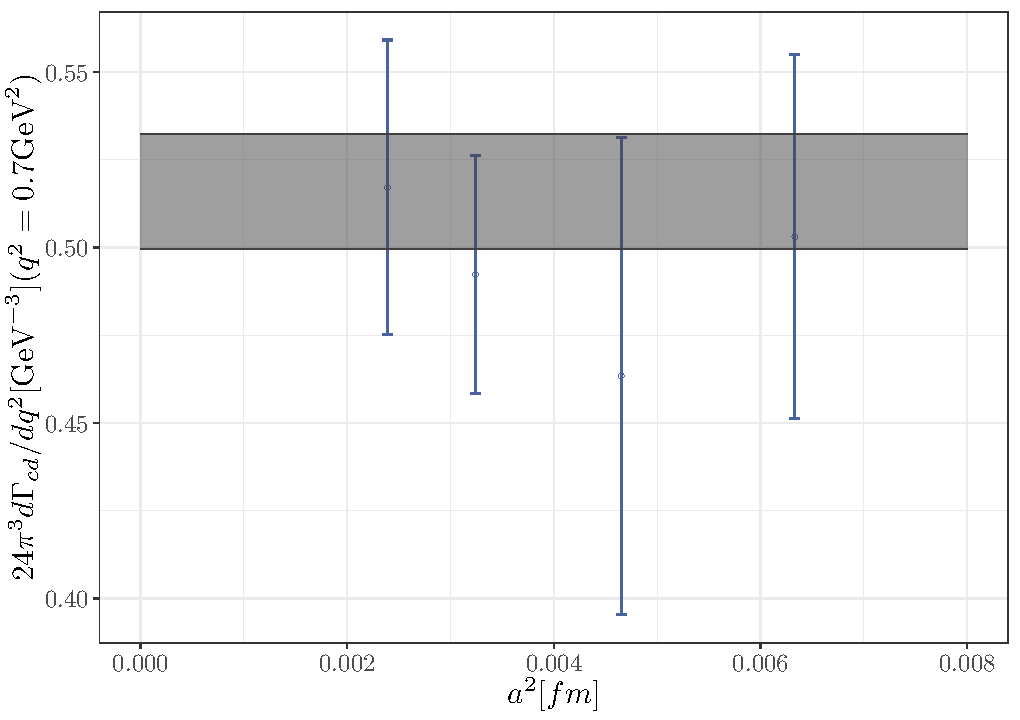
\includegraphics[scale=0.7]{figures/dGamma_continuum_th9.pdf}
		\caption{Continuum limit of $d\Gamma_{cd}/dq^2 $ for the channel $cd$}
		\label{fig:dGamma_continuum}
	\end{center}
\end{figure}

Finally a comparison of the contribution from the two different channels is shown in Figure~\ref{fig:gamma_cs_cd}, were we observe that once we multiply the contribution by its own CKM matrix element the $cd$ contribution is suppressed.

\begin{figure}
	\begin{center}
		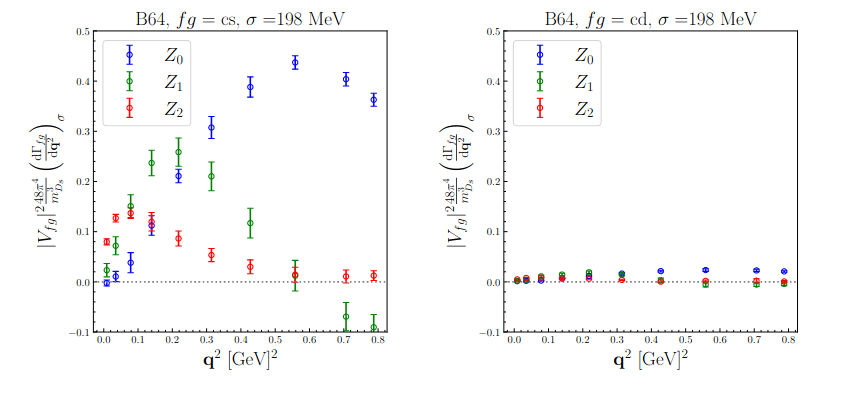
\includegraphics[scale=0.6]{figures/Screenshot from 2024-07-27 19-31-31.png}
		\caption{Comparison of the decay width for the $cs$ channel on the left and $cd$ channel on the right. The three contribution to the decay rate of Eq.~(\ref{eq:gamma}) are showed separatly labeled as $Z_0$, $Z_1$ and $Z_2$.}
		\label{fig:gamma_cs_cd}
	\end{center}
\end{figure}

In the remaining time of the project we will focus on computing the $su$ channel and verifying the
theoretical expectation that it suppressed. Further we will do extra run to check the effect of an
eventual mistuning of the quark mass of the charm and strange as well as finalizing the analysis and prepare a publication.

% For the quark-gluon momentum fraction in the pion (and kaon) we have
% generated data according to plan. More specifically, we have generated
% light loops for the ensemble cD211.054.96 using hierarchical and
% spin-color dilution. Second, we have generated meson two-point
% functions for the same esemble using stochastic sources and spin
% dilution. Third, we have been generating two-point functions for
% mesons and baryons for the cD211.054.96 ensemble using point sources
% and smearing.



% \subsubsection{$\langle x\rangle$ of the pion and kaon}

% \begin{figure}
% 	\subfigure{\includegraphics[width=.45\textwidth,page=1]{./figures/plot_ratio_alltseq_xq-conn-oet_cD96_l-gd-ls-gi_cvc.pdf}}\quad
% 	\subfigure{\includegraphics[width=.45\textwidth,page=6]{./figures/plot_ratio_alltseq_xq-conn-oet_cD96_l-gd-ls-gi_cvc.pdf}}\quad
% 	\subfigure{\includegraphics[width=.45\textwidth,page=1]{./figures/plot_ratio_alltseq_xq-conn-oet_cD96_s-gd-sl-gi_cvc.pdf}}\quad
% 	\subfigure{\includegraphics[width=.45\textwidth,page=6]{./figures/plot_ratio_alltseq_xq-conn-oet_cD96_s-gd-sl-gi_cvc.pdf}}\quad
% 	%%%  
% 	\caption{Results for the ratio determining the connected contribtuion to the bare $\langle x\rangle^K$ in the kaon on
% 		ensemble cD211.054.96. Top row shows the light quark operator insertion, bottom row for the strange quark.
% 		The left column uses zero hadron momentum and the $T^{q}_{44}$  tensor component of the quark EMT,
% 		the right one $|\Pvec| = 2\pi/L$ and component $T^{q}_{4k}$.
% 		We demonstrate the saturation for a sequence of increasing source-sink separations $\Delta t_{fi}$.}
% 	\label{fig:resultx-conn}
% \end{figure}


% \begin{figure}
% 	\subfigure{\includegraphics[width=.45\textwidth,page=3]{./figures/plot_disc_ratio_xq-kaon-ll_cD96.pdf}}\quad
% 	\subfigure{\includegraphics[width=.45\textwidth,page=3]{./figures/plot_disc_ratio_xq-kaon-ss_cD96.pdf}}\quad
% 	\subfigure{\includegraphics[width=.45\textwidth,page=3]{./figures/plot_disc_ratio_xq-kaon-cc_cD96.pdf}}\quad
% 	\subfigure{\includegraphics[width=.45\textwidth,page=9]{./figures/plot_gluon_ratio_xg-kaon_clover_cD96.pdf}}\quad
% 	%%%  
% 	\caption{Results for the ratio determining the disc-connected contribtuions to the bare $\langle x\rangle^K$ in the kaon on
% 		ensemble cD211.054.96. Top row shows the light and strange quark operator insertions,
% 		bottom left the charm quark case; bottom right we show the ratio for the gluon EMT insertion in the kaon using 10 steps of stout smearing.}
% 	\label{fig:resultx-disc}
% \end{figure}

% So far, a lattice QCD computation of the quark and gluon contributions
% to $\langle x\rangle$ in the pion was not available. Here we present
% first such results at a single value of the lattice spacing but with
% physical value of the pion mass.

% The relevant traceless elements of the Euclidean Energy-Momentum
% tensor
% for quark flavour $q$ with the symmetrised covariant derivative
% $\stackrel{\leftrightarrow}{D}_\mu$ reads
% \begin{equation}
% 	\begin{split}
% 		\bar{T}_{4k}^q\ &=\ -\frac{i}{4}\bar q\left(\gamma_4\stackrel{\leftrightarrow}{D}_k + \gamma_k
% 		\stackrel{\leftrightarrow}{D}_4\right)q\,,\\
% 		\bar{T}_{44}^q\ &=\ -\frac{1}{2}\bar q\gamma_4
% 		\stackrel{\leftrightarrow}{D}_4\, q - \mathrm{traces}\,.
% 	\end{split}
% \end{equation}
% Analogously, for the gluon one finds
% \begin{equation}
% 	\bar{T}^g_{\mu\nu} \ =\ F^{\{\mu\rho}_{~}F^{\nu\}}_\rho- \mathrm{traces}\,,
% \end{equation}
% where $\{\ldots\}$ means symmetrisation over the indices.
% Then one obtains for $X=q, g$ the corresponding contribution to
% $\langle x\rangle$ from
% \begin{equation}
% 	\langle P(\mathbf{p})|\bar{T}^X_{\mu\nu}| P(\mathbf{p})\rangle\ =\
% 	2\langle x\rangle^X_P\left(p_\mu p_\nu - \delta_{\mu\nu}\frac{p^2}{4}\right)\,,
% \end{equation}
% where $P$ stands for pion or kaon.
% These matrix elements can be extracted from a ratio of Euclidean
% three- and two-point functions
% \begin{equation}
% 	R^X_P(t, t_f, t_i)\ =\ \frac{\langle P(t_f,\vec
% 	p)\,\bar{T}^X_{\mu\nu}(t)\, P(t_i,\vec p)\rangle}
% 	{\langle P(t_f,\vec p)\ P(t_i,\vec p)}
% \end{equation}
% which are related to the aforementioned matrix elements via
% \begin{equation}
% 	R^X_P(t, t_f, t_i)\to
% 	\frac{1}{2E_P}\frac{\langle P(\mathbf{p})|\bar{T}^X_{\mu\nu}| P(\mathbf{p})\rangle}{1+\exp(-E_P(T
% 	- 2(t_f-t_i)))}\,.
% \end{equation}
% for $t_f - t_i$ and $t$ large enough such that excited states have
% decayed sufficiently.

% We have published results for the full flavour decomposition of the
% momentum fraction of quarks and gluons in the pion in
% PRL~\cite{OExtendedTwistedMass:2021rdx}. In this publication we could
% for the first time present results for the momentum fraction of the
% light, strange and charm quarks and the gluons in the pion, taking the
% mixing under renormalisation into account. Most importantly, in this
% way we could check whether all contributions to $\langle x\rangle$ sum
% up to one, which they do in our case within errors. Still, further
% investigations will be needed to further reduce the error and to
% understand the relatively large gluon contribution we obtained.

% For the other ensembles and observables the analysis of the data is
% currently ongoing. In \cref{fig:resultx-conn} we show preliminary results for the kaon
% connected only contribution for light ($\bar u u$) and strange ($\bar
% 	s s$) quarks for different source-sink separations. A clear plateau
% becomes visible for large enough source-sink separations.

% In \cref{fig:resultx-disc} we show preliminary results for the
% corresponding disconnected contributions again for the kaon. These are
% extracted from $T_{4k}$. While in the upper two panels and the lower
% left one we show the light, strange and charm quark contributions,
% respectively, the gluon contribution is displayed in the lower right
% panel. We show the results for different source-sink separations.

\subsection{Sub-project 2: decay constant $f_D$ and $f_{D_s}$}

The decay
constant of the corresponding pseudo-scalar (PS) meson can be extracted from the equation
\begin{equation}
	f_\mathrm{PS}=(\mu_f+\mu_{f'})\frac{\langle 0| P_{ff'}|
		\mathrm{PS}\rangle}{M_\mathrm{PS}^{ff'}\sinh(M_\mathrm{PS}^{ff'})}\,
\end{equation}
where the matrix element is extracted from the correlation function
$\langle O_\mathrm{PS}(t)O_\mathrm{PS}(t)^\dagger \rangle$  at large time separations. The PS-meson is made out of
valence quark flavours with bare masses $\mu_f$ and $\mu_{f'}$ ,
its mass is denoted by $M_\mathrm{PS}^{ff'}$ and the corresponding interpolating
operator is $O_\mathrm{PS}=\bar f \gamma_5 f' $ . We plan to compute the
decay constant for the $D_s$ and $D$ meson, thus $f=c$ and $f'=s,d$.

We produced all the data necessary to extract the decay constant for all the ensemble listed in
Table~\ref{tab:ensembles}, but so far the data were not analyzed yet.
We  concentrate our effort in the analysis of the decay rate of the sub-project-1 which is
close to be completed and we will analyze $f_D$ and $f_{D_s}$ in the remaining time of the project.

% For the hadronic vacuum polarization function we have also generated
% data according to our plan. Here we have generated meson two-point
% function for the finer lattice spacing ensemble cC211.06.80 using
% stochastic sources and spin dilution.

% A first account for our work on the hadronic vacuum polarization has
% recently appeared on the arXiv~\cite{OAlexandrou:2022amyw}. While not
% yet peer reviewed, it has already gained nine citations as of August
% 15 in the few weeks it is online. In this paper we present a lattice
% determination of the leading-order hadronic vacuum polarization (HVP)
% contribution to the muon anomalous magnetic moment, $a_{\mu}^{\rm
% 			HVP}$, in the so-called short and intermediate time-distance
% windows, $a_{\mu}^{SD}$ and $a_{\mu}^W$, defined by the RBC/UKQCD
% Collaboration\,\cite{RBC:2018dos}. The computation is performed using
% $N_f=2+1+1$ flavour lattice QCD with the continuum limit taken with
% three values of the lattice spacing.

% We use the RBC/UKQCD collaboration proposal to write
% \begin{equation}
% 	a_\mu^\textrm{HVP} = a_\mu^\mathrm{SD} + a_\mu^\mathrm{W} + a_\mu^\mathrm{LD}
% \end{equation}
% which separately probe short-distance (SD), intermediate- (W) and
% long-distance (LD) physics. For the exact definition we refer to
% Rev.~\cite{RBC:2018dos} or our publication~\cite{OAlexandrou:2022amyw}.

% For the short distance window we obtain $a_\mu^\mathrm{SD}({\rm ETMC}) =
% 	69.33\,(29) \cdot 10^{-10}$, which is consistent with the recent
% dispersive value $a_\mu^\mathrm{SD}(e^+ e^-) = 68.4\,(5) \cdot
% 	10^{-10}$\,\cite{Colangelo:2022vok} within $\simeq 1.6 \, \sigma$. In
% the case of the intermediate window we get the value $a_\mu^W({\rm
% 			ETMC}) = 235.0\,(1.1) \cdot 10^{-10}$, which is consistent with the
% result $a_\mu^W({\rm BMW}) = 236.7\,(1.4) \cdot
% 	10^{-10}$\,\cite{Borsanyi:2020mff} by the BMW collaboration as well as
% with the recent determination by the CLS/Mainz group of  $a_\mu^\mathrm{W}({\rm
% 		CLS}) = 237.30\,(1.46) \cdot 10^{-10}$ \,\cite{Ce:2022kxy} at the
% $\sim 1.0 - 1.3 \, \sigma$ level. However, it is larger than the
% dispersive result $a_\mu^\mathrm{W}(e^+ e^-) = 229.4\,(1.4) \cdot
% 	10^{-10}$\,\cite{Colangelo:2022vok} by $\simeq 3.1 \, \sigma$. The
% tension increases to $\simeq 4.2 \, \sigma$ if we average our ETMC
% result with the BMW and the CLS/Mainz ones. Our accurate lattice
% results in the short and intermediate windows hint at possible
% deviations of the $e^+ e^-$ cross section data with respect to
% Standard Model (SM) predictions distributed somewhere in the low (and
% possibly intermediate) energy regions, but not in the high energy
% region.

% \begin{figure}[htb!]
% 	\begin{center}
% 		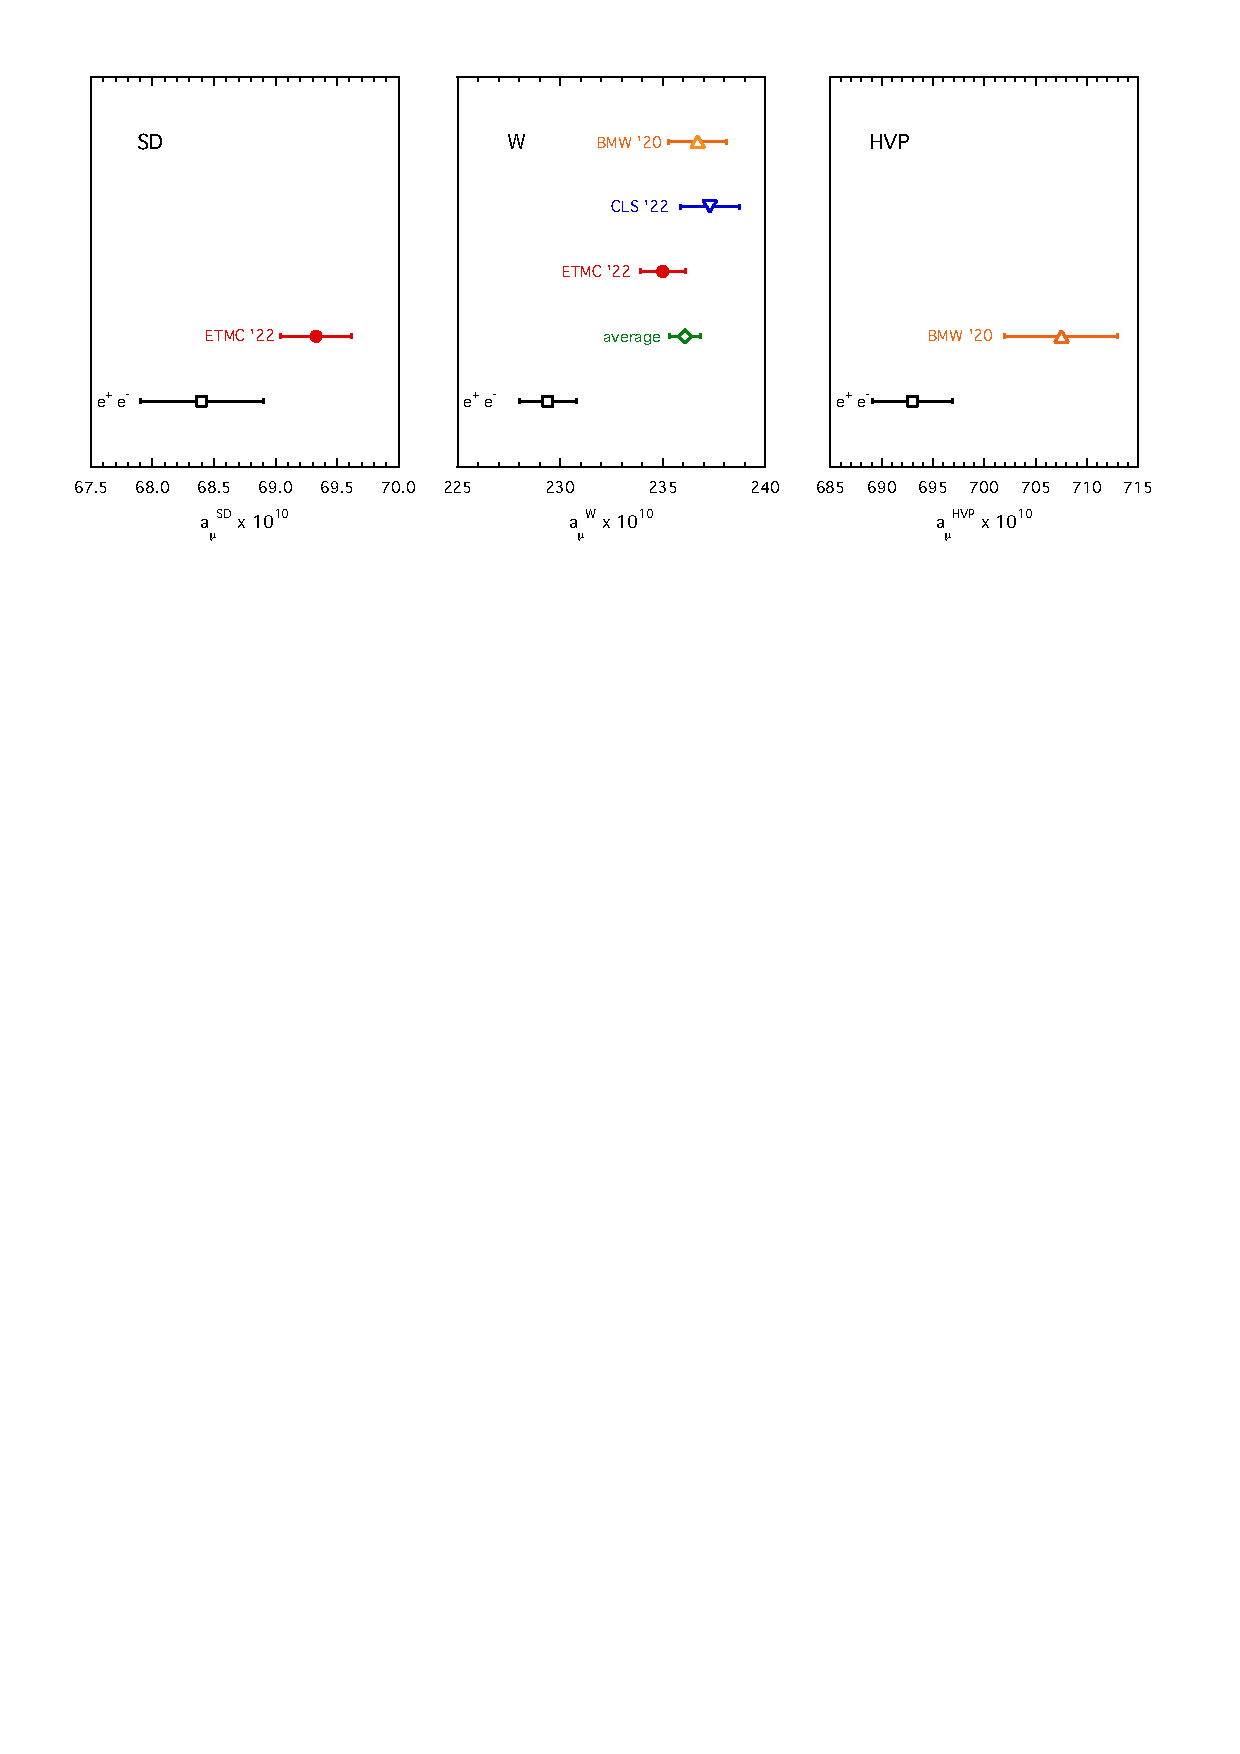
\includegraphics[scale=0.85]{figures/comparisons}
% 		\caption{\it \small We show lattice QCD results of the
% 			short-distance window $a_\mu^{\rm SD}$ (left panel),
% 			intermediate window $a_\mu^{\rm W }$ (central panel), obtained
% 			in this work and in Refs.\,\cite{Borsanyi:2020mff,Ce:2022kxy},
% 			and the full HVP term $a_\mu^{\rm HVP}$ (right panel) from
% 			Ref.\,\cite{Borsanyi:2020mff}, compared with the corresponding
% 			dispersive determinations from Ref.\,\cite{Colangelo:2022vok},
% 			based on experimental $e^+ e^- \to$ hadrons data. In the central
% 			panel, the green diamond denotes the average of our result with
% 			those from
% 			Refs.\,\cite{Borsanyi:2020mff,Ce:2022kxy}, namely $a_\mu^{\rm W}
% 				= 236.08 (74) \cdot 10^{-10}$.}
% 		\label{fig:comparison}
% 	\end{center}
% \end{figure}

% This result is visualised in \cref{fig:comparison} taken from our
% publicaiton~\cite{OAlexandrou:2022amyw}: in the leftmost panel of this
% figure we compare our lattice result for the short-distance (SD) window
% $a_\mu$ with the dispersive determination from
% Ref.~\cite{Colangelo:2022vok}. In the middle panel the same comparison
% is performed for the intermediate window (W) definition, this time also
% comparing to other available lattice results for this quantity. The
% systematic deviation from the dispersive determination becomes nicely
% visible. In the rightmost panel the full hadronic vacuum polaristaion
% (HVP) is shown, comparing the lattice determination by the BMW
% collaboration~\cite{Borsanyi:2020mff} with the dispersive
% determination.

% If confirmed, this deviation in the intermediate window might provide
% a hint for new, beyond the standard model physics. However, even
% better control of systematic effects is needed, which will be explored
% in the new computer time proposal we are submitting.

%\subsubsection{${\cal   F}_{\pi^0\rightarrow \gamma^{(*)}
%    \gamma^{(*)}}$ of the pion}


\section{Realization of the project}
\rule{\textwidth}{0.4pt}\\


we have produced data running from 2 to 56 nodes depending on the ensemble
on Juwels Booster. The two sub-project shares the same run. We manage to optimize the
memory footprint of our code nissa~\footnote{\url{https://github.com/sunpho84/nissa}} being 
able to reduce the number of nodes used for the run in of the ensemble cB211.072.64 from 8 to 4 
and the nodes necessary to simulate the ensemble cC211.06.80 form 20 to 10, resulting in a more efficient run.

% In detail, we have run
% \begin{itemize}
% 	\item Sub-project 1:
% 	      For this sub-project we have also significantly developed our code
% 	      base by moving from a code with inversions on the GPU and
% 	      contractions on the CPU to both on the GPU now: all the contractions
% 	      of the operators relevant for moments of parton distribution
% 	      functions $\langle x^n\rangle\,,\ n<4$ are implemented in the plegma
% 	      software now.
% 	\item Sub-project 2: due to the slighly smaller lattice volume
% 	      we were running using 20 nodes of Juwels Booster.
% \end{itemize}


\section{Publications with the appropriate acknowledgement}
\rule{\textwidth}{0.4pt}

We are preparing a publication with our result of the inclusive decay rate $D_s\to X\ell\nu$ and 
preliminary result were presented at the Lattice conference 2024


\begin{thebibliography}{99}
	%\makeatletter
	%\renewcommand\@bibitem[1]{\item\if@filesw \immediate\write\@auxout
	%    {\string\bibcite{#1}{O\the\value{\@listctr}}}\fi\ignorespaces}% <------------
	%\def\@biblabel#1{[O#1]}% <-------------------
	%\makeatother
	%\cite{Hansen:2019idp}
	\bibitem{Hansen:2019idp}
	M.~Hansen, A.~Lupo and N.~Tantalo,
	%``Extraction of spectral densities from lattice correlators,''
	Phys. Rev. D \textbf{99} (2019) no.9, 094508
	doi:10.1103/PhysRevD.99.094508
	[arXiv:1903.06476 [hep-lat]].
	%85 citations counted in INSPIRE as of 27 Jul 2024

	\bibitem{talk1}
	Talk at the Lattice conference 2024, University of Liverpool, United Kingdom, from July 28th to August 3rd, 2024.
	"Inclusive semileptonic $D_s\mapsto X \ell \nu$ decay from lattice QCD" by A.~De~Santis, ID-387.

	\bibitem{talk2}
	Talk at the Lattice conference 2024, University of Liverpool, United Kingdom, from July 28th to August 3rd, 2024.
	"Semileptonic Inclusive Decay of the $D_s$ Meson" by C.~Gro\ss, ID-140.

	%\cite{Alexandrou:2022amy}
	% \bibitem[O1]{OAlexandrou:2022amyw}
	% C.~Alexandrou, S.~Bacchio, P.~Dimopoulos, J.~Finkenrath, R.~Frezzotti, G.~Gagliardi, M.~Garofalo, K.~Hadjiyiannakou, B.~Kostrzewa and K.~Jansen, \textit{et al.}
	% %``Lattice calculation of the short and intermediate time-distance hadronic vacuum polarization contributions to the muon magnetic moment using twisted-mass fermions,''
	% [arXiv:2206.15084 [hep-lat]].
	%8 citations counted in INSPIRE as of 11 Aug 2022

	%\cite{ExtendedTwistedMass:2021rdx}
	\bibitem[O2]{OExtendedTwistedMass:2021rdx}
	C.~Alexandrou \textit{et al.} [Extended Twisted Mass],
	%``Quark and Gluon Momentum Fractions in the Pion from Nf=2+1+1 Lattice QCD,''
	Phys. Rev. Lett. \textbf{127} (2021) no.25, 252001
	doi:10.1103/PhysRevLett.127.252001
	[arXiv:2109.10692 [hep-lat]].
	%1 citations counted in INSPIRE as of 11 Aug 2022

\end{thebibliography}


\section{Theses completed within the project}
\rule{\textwidth}{0.4pt}

There are no thesis yet to report.

\section{Additional references}
\rule{\textwidth}{0.4pt}

\bibliography{biblio}

\section{Material suitable for the general public}
\rule{\textwidth}{0.4pt}

Currently, we do not yet have such material available.

\section{Usage of Additional Computer Resources}

We did not use additional computer resources.
% Thanks to the availability of using additional resources within the
% low-priority queue, our group was able to use double of the requested
% time for the project. Namely, we have used 41.44 Mcore-hrs compared to
% the 20.20 Mcore-hrs requested. These resources have allowed us to
% significantly increase the scientific impact of the project and we are
% extremely grateful to JSC for allowing this. Namely, they have enabled
% us to accumulate larger statistics than planned and to perform
% additional calculations.

% Of course, as jobs in the low-priority queue are not guaranteed to
% run, we have mostly used these resources for additional statistics and
% for projects we were planning to do later. We recall that we are
% working with ensembles at the physical point at three values of the
% lattice spacing. Below, in the ensemble names the lattice spacing is
% encoded at the beginning of the ensemble name as cB, cC and cD,
% respectively.

% In the following we give a detailed account of how we used the
% additional resources. The following table is an update of the
% corresponding table from our original application and can be
% compared. Sub-project 3 and Sub-project 4 are new and were not yet
% present in the original proposal.

% \begin{center}
% 	{\small
% 		\begin{tabular}{lllccccr} \hline\hline
% 			Sub-             &
% 			Type             &
% 			Problem          &
% 			\# runs          &
% 			\# steps/        &
% 			Wall time/       &
% 			\# cores/        &
% 			Total                                                           \\
% 			project          &
% 			of run           &
% 			size             &
% 			                 &
% 			run              &
% 			step [hours]     &
% 			run              &
% 			[core-h]                                                        \\
% 			\hline\hline
% 			%%%%
% 			%%%%
% 			%%%%
% 			1                &
% 			(1)              &
% 			$96^3\times 192$ &
% 			500              &
% 			8                &
% 			5.3              &
% 			24 nodes         &
% 			$24.423 \times 10^6$                                            \\
% 			%%%%
% 			%%%%
% 			%%%%
% 			~                &
% 			(2)              &
% 			~                &
% 			500              &
% 			1                &
% 			5.5              &
% 			24 nodes         &
% 			$3.168 \times 10^6$                                             \\
% 			%%%%
% 			%%%%
% 			%%%%
% 			~                &
% 			(3)              &
% 			~                &
% 			500              &
% 			1                &
% 			5.6              &
% 			24 nodes         &
% 			$3.227 \times 10^6$                                             \\
% 			%%%
% 			%%% extension for cB211 physical point, for x_q disc, p2gg P-disc, V-disc VV-disc
% 			%%%
% 			2                &
% 			(4)              &
% 			$80^3\times 160$ &
% 			400              &
% 			1                &
% 			4.3              &
% 			20 nodes         &
% 			$1.652 \times 10^6$                                             \\
% 			%%%
% 			%%%
% 			%%%
% 			3                &
% 			(5)              &
% 			$96^3\times 192$ &
% 			600              &
% 			1                &
% 			8.4              &
% 			24 nodes         &
% 			$5.808 \times 10^6$                                             \\
% 			4                &
% 			(6)              &
% 			$96^3\times 192$ &
% 			500              &
% 			1                &
% 			5.4              &
% 			24 nodes         &
% 			$3.112 \times 10^6$                                             \\
% 			\hline\hline
% 			TOTAL            &   &  &  &  &  &  & $41.4 \times 10^6$ core-h \\
% 		\end{tabular}
% 	}
% \end{center}

% Changes and additional items are explained in the following:
% \begin{description}
% 	\item[Sub-project 1:] the statistics has been increased from 300 to 500 configurations (``\# runs'' in the table). This has been performed for all type of runs (1-3) and it accounts of 53\% of the additional resources.
% 	\item[Sub-project 2:] No changes apply to this sub-project.
% 	\item[Sub-project 3:] Meson two-point functions for computing the hadronic vacuum polarisation contributions to the muon magnetic moment, presented in Ref.~\cite{OAlexandrou:2022amyw}, have been calculated also for the cB211.072.96 ensemble. This is listed as type of run (5) and it complements similar calculations performed for the cD211.054.96 ensemble, listed as 1(3), and for the cC211.06.80 ensemble, listed as 2(4). This additional ensemble has been used for studying finite-size effects and higher statistics has been required compared to the cD211.054.96 ensemble. Namely 600 configurations have been used and 50\% more statistics has been accumulated per configuration.
% 	\item[Sub-project 4:] On the cD211.054.96 ensemble we have computed also connected 2- and 3-point functions for a complete evaluation of the
% 		quark and gluon momentum fractions $\langle x\rangle^{\pi/K}_{q/g}$ for pion and kaon. The insertion of the quark energy momentum tensor into
% 		the pion or kaon 2-point correlator produces both connected and disconnected 3-point functions. The bulk of computational effort goes
% 		into the loop calculations for the disconnected, covered in run type 1. Within the additional resources we were able to finalise our data production
% 		for the pion and kaon 2-point functions to calculate the disconnected contributions for quark and even gluon energy-momentum tensor
% 		as in Ref.~\cite{OExtendedTwistedMass:2021rdx}. This data set was not already covered by the run types 2-4, due to the combination of using 96 stochastic
% 		time-slice sources with zero and non-zero momentum, and with source and sink smearing.\\
% 		Finally, the additional resources allowed for computing the
% 		fully connected 3-point functions for $\langle x\rangle_{q}$ for both pion and kaon.
% 		As a result we have a complete computation of the quark and gluon momentum fraction for pion and kaon on ensemble cD211.054.96, and together
% 		already existing data from the two coarser lattices cB211.072.64 and cC211.06.80 we now extrapolate the momentum fractions
% 		to the continuum at physical pion mass.
% 		A corresponding publication is in preparation.

%\end{description}

In conclusion, the runs for the ensembles $cB211.072.48(64,96)$ were necessary to control the 
finite volume effects on our obervable while the other run were necessary to control the continuum 
limit.
Our preliminary result obtained looks very promising and a paper is under preparation. 

% the runs of type (1,2,4,5) have been critical in
% accumulating all the statistics required for the our work on the
% hadronic vacuum polarisation published in
% Ref.~\cite{OAlexandrou:2022amyw} (highly cited since June 2022). The
% runs (1,3,6) are part of our effort on extending the work presented in
% Ref.~\cite{OExtendedTwistedMass:2021rdx} for one ensemble, to three
% physical point ensembles and taking the continuum limit. Finally, the
% results produced in (1) will also be used for computing the
% disconnected contributions in many other quantities.

The results obtained with these resources have also been presented
in different talks at the International Symposium on Lattice Field
Theory in August of this year in Liverpool, UK.



\end{document}
